\documentclass[12pt,a4paper]{article}
\usepackage[
	top=35mm,
	left=25mm,
	right=25mm,
	bottom=25mm,
	headheight=55pt,
	footskip   = 10pt,
]{geometry}
%\usepackage{t1enc}
\usepackage{lmodern} % pdflatex or dvi latex
\usepackage[T1]{fontenc}
\usepackage[utf8]{inputenc}

\usepackage{fontspec}
\setmainfont{Times New Roman}
%\setmainfont{Raleway-Regular}
\usepackage[mathscr]{eucal}
\usepackage[magyar]{babel}
\usepackage{amssymb}
\usepackage{amsthm}
\usepackage{graphics}
\usepackage{amsxtra}
\usepackage{microtype}
\usepackage[absolute,overlay]{textpos}
\usepackage{array}

\usepackage{xcolor}

\newcolumntype{M}[1]{>{\centering\arraybackslash}m{#1}}
\newcolumntype{N}{@{}m{0pt}@{}}



\setlength{\parindent}{0pt}
%fejléc-----------------------------------------------------------------------

\usepackage{fancyhdr}
\usepackage[most]{tcolorbox}
\usepackage{color, colortbl}

\usepackage{setspace}
\usepackage{enumitem}    

%functions-----------------------------------------------------------------------
\DeclareMathOperator{\arccot}{arccot}
\DeclareMathOperator{\arctg}{arctg}
\DeclareMathOperator{\arcctg}{arcctg}
\DeclareMathOperator{\tg}{tg}
\DeclareMathOperator{\ctg}{ctg}


%checkbox, dotfill------------------------------------
\newcommand{\checkbox}{$\square$}
\newcommand\fillin[1][3cm]{\makebox[#1]{\dotfill}}
\newcommand\fillinlong{................................................. }
\newcommand\fillinshort{........}
\newcommand\dunderline[3][-1pt]{{%
  \sbox0{#3}%
  \ooalign{\copy0\cr\rule[\dimexpr#1-#2\relax]{\wd0}{#2}}}}
  




%header and footer---------------------------------------------

\fancypagestyle{face}{%
\fancyhf{}
\renewcommand{\headrulewidth}{1pt}

\fancyhead[R]{%
%  \scshape
  \color{black}
Név: \fillinlong osztály:\fillinshort
\vspace{10pt}
}

\renewcommand{\footrulewidth}{1pt}
%\fancyfoot[L]{\vspace{0.2cm}\includegraphics[scale=.2]{mp_presentation_logo}}
\fancyfoot[L]{Matematika}
\fancyfoot[R]{
\vspace{-10pt}
\begin{spacing}{2pt}
középszint — írásbeli vizsga 1811 \\ I. összetevő  
\end{spacing}}
}

\fancypagestyle{first}{%
\fancyhf{}
\renewcommand{\headrulewidth}{1pt}

\fancyhead[L]{%
%  \scshape
  \color{black}
Matematika\\
középszint}
\fancyhead[R]{%
%  \scshape
  \color{black}
Név: \fillinlong osztály:\fillinshort
\vspace{4pt}
}

\renewcommand{\footrulewidth}{1pt}
%\fancyfoot[L]{\vspace{0.2cm}\includegraphics[scale=.2]{mp_presentation_logo}}
\fancyfoot[L]{\vspace{0.2cm}1811 írásbeli vizsga I. összetevő} 
\fancyfoot[C]{\vspace{0.2cm} \thepage\hspace{2pt} / \hspace{2pt}\pageref{LastPage}}   
\fancyfoot[R]{\vspace{0.2cm}2018. május 8.}  
}


\usepackage{pgfplots}
\usepackage{tikz}
%tikz library setup------------------------------------
\usetikzlibrary{arrows,positioning,shapes,fit,calc}
\usetikzlibrary{arrows.meta,shadings,bending}
\usetikzlibrary{shapes.geometric,positioning}
\usetikzlibrary{math, shapes.misc}
\usetikzlibrary{intersections}
\usetikzlibrary{backgrounds}
\usetikzlibrary{decorations.pathreplacing} 
\usepgfplotslibrary{fillbetween}
\usetikzlibrary{decorations.pathmorphing,shadows}
\usetikzlibrary{angles,quotes}

\pgfplotsset{compat=1.14}


\begin{document}

\pagestyle{face}
\begin{Huge}
    \begin{textblock*}{0cm}(2.4cm,4cm)
        \rotatebox{90}{\textls[120]{\textbf{{\fontsize{30pt}{0pt}\selectfont \dunderline[-2pt]{3pt}{ÉRETTSÉGI VIZSGA • 2018. május 8.}}}}}
    \end{textblock*}
    \begin{center}
        \vspace*{3cm}
        \fontsize{28pt}{0pt}\selectfont 
        \textbf{MATEMATIKA} \\
        \vspace*{2cm}
        \textbf{KÖZÉPSZINTŰ \\ ÍRÁSBELI VIZSGA} \\
        \vspace*{1cm}
        \fontsize{26pt}{0pt}\selectfont 
        \textbf{2018. május 8. 8:00 } \\
        \vspace*{1cm}
        \fontsize{30pt}{0pt}\selectfont 
        \textbf{I.}\\
        \vspace*{1.5cm}
        \fontsize{22pt}{0pt}\selectfont 
        Időtartam: 45 perc \\
        \vspace*{\fill}
        \fontsize{18pt}{0pt}\selectfont 
        \textbf{EMBERI ERŐFORRÁSOK MINISZTÉRIUMA}
    \end{center}
    
    \fontsize{16pt}{4pt}\selectfont 
    \begin{textblock*}{0pt}(13cm,20cm)
    
    \setlength\extrarowheight{12pt}

% https://tex.stackexchange.com/questions/159257/increase-latex-table-row-height
    
    \begin{table}[ht]
    \begin{tabular}{|cl|}
    \hline
    \multicolumn{2}{|M{6cm}|}{Pótlapok száma} \\[2pt]
    \hline
    \multicolumn{1}{|c|}{Tisztázati}  &  \\[2pt]
    \hline
    \multicolumn{1}{|c|}{Piszkozati}  &  \\[2pt]
    \hline
    \end{tabular}
    \end{table}
    
    \end{textblock*}
\end{Huge}
\newpage

\pagestyle{first}

\fontsize{12.5pt}{0pt}\selectfont 

\begin{center}
\LARGE \textbf{Fontos tudnivalók}\par
\end{center}
\vspace{1cm}
\begin{enumerate}[leftmargin=*,itemsep=0.9cm ]

  \item
  A feladatok megoldására 45 percet fordíthat, az idő leteltével a munkát be kell fejeznie.
  \item
  A megoldások sorrendje tetszőleges. 
  \item
  A feladatok megoldásához szöveges adatok tárolására és megjelenítésére nem alkalmas zsebszámológépet és bármilyen négyjegyű függvénytáblázatot használhat, más elektronikus vagy írásos segédeszköz használata tilos! 
  \item
  \textbf{A feladatok végeredményét az erre a célra szolgáló keretbe írja}, a megoldást csak akkor kell részleteznie, ha erre a feladat szövege utasítást ad! 
  \item 
  A dolgozatot tollal írja, az ábrákat ceruzával is rajzolhatja. Az ábrákon kívül a ceruzával írt
részeket a javító tanár nem értékelheti. Ha valamilyen megoldást vagy megoldásrészletet
áthúz, akkor az nem értékelhető. 
\item 
Minden feladatnak csak egy megoldása értékelhető. Több megoldási próbálkozás esetén
egyértelműen jelölje, hogy melyiket tartja érvényesnek! 
\item 
Kérjük, hogy \textbf{a szürkített téglalapokba semmit ne írjon!} 
\end{enumerate}

\newpage
\begin{enumerate}[leftmargin=*,label=\textbf{\large\arabic*.}]
    \item 
    Egy 80 grammos csokoládé tömegének 35 százaléka kakaó. Hány gramm kakaó van ebben a csokoládéban? 

    \vspace{4cm}
    
    \begin{flushright}
        \begin{tabular}{|M{6cm}|M{2cm}|M{2cm}|N}
        \hline
        \vspace{20pt}
        \hspace{1cm}gramm
         & 
        \vspace{20pt}
         2 pont \cellcolor{black!20} & \cellcolor{black!20} \\[30pt]
        \hline
        \end{tabular}
    \end{flushright}

    \item
    Írja fel a {2; 3; 4} halmaznak azokat a részhalmazait, melyeknek a 2 eleme és a 4 nem
eleme! 
    \vspace{4cm}

    \begin{flushright}
        \begin{tabular}{|M{6cm}|M{2cm}|M{2cm}|N}
        \hline
         & 
        \vspace{20pt}
         2 pont \cellcolor{black!20} & \cellcolor{black!20} \\[30pt]
        \hline
        \end{tabular}
    \end{flushright}


    \item
    Ma kedd van. A hét melyik napja lesz 100 nap múlva? 
    \vspace{4cm}

    \begin{flushright}
        \begin{tabular}{|M{6cm}|M{2cm}|M{2cm}|N}
        \hline
         & 
        \vspace{20pt}
         2 pont \cellcolor{black!20} & \cellcolor{black!20} \\[30pt]
        \hline
        \end{tabular}
    \end{flushright}

\newpage

    \item
    Egy 100 cm \(\times\) 50 cm \(\times\) 50 cm belső méretű (téglatest alakú) akváriumot vízzel töltünk fel.
Mennyibe kerül a feltöltéshez szükséges víz, ha 1 köbméter víz ára 220 Ft? \\
Megoldását részletezze! 
    \vspace{4cm}
    
    \begin{flushright}
        \begin{tabular}{|>{\raggedleft}M{6cm}|M{2cm}|M{2cm}|}
        \cline{2-3}
        \multicolumn{1}{c|} \
         & 
        \vspace{20pt}
         2 pont \cellcolor{black!20} & \cellcolor{black!20} \\[30pt]
        \hline
        \vspace{20pt}
        Ft-ba kerül. 
        & 
        \vspace{20pt}
         1 pont \cellcolor{black!20} & \cellcolor{black!20} \\[30pt]
        \hline
        \end{tabular}
    \end{flushright}


    \item
Egy héttagú társaság hat tagjáról tudjuk, hogy hány ismerőse van a társaságban: 1, 2, 3,
4, 4, 5. Rajzoljon erről a társaságról egy lehetséges ismeretségi gráfot, és adja meg a hetedik ember (\(G\)) ismerőseinek számát ebben az esetben! (Az ismeretségek kölcsönösek.) 
    \begin{figure}[h]
        \centering
        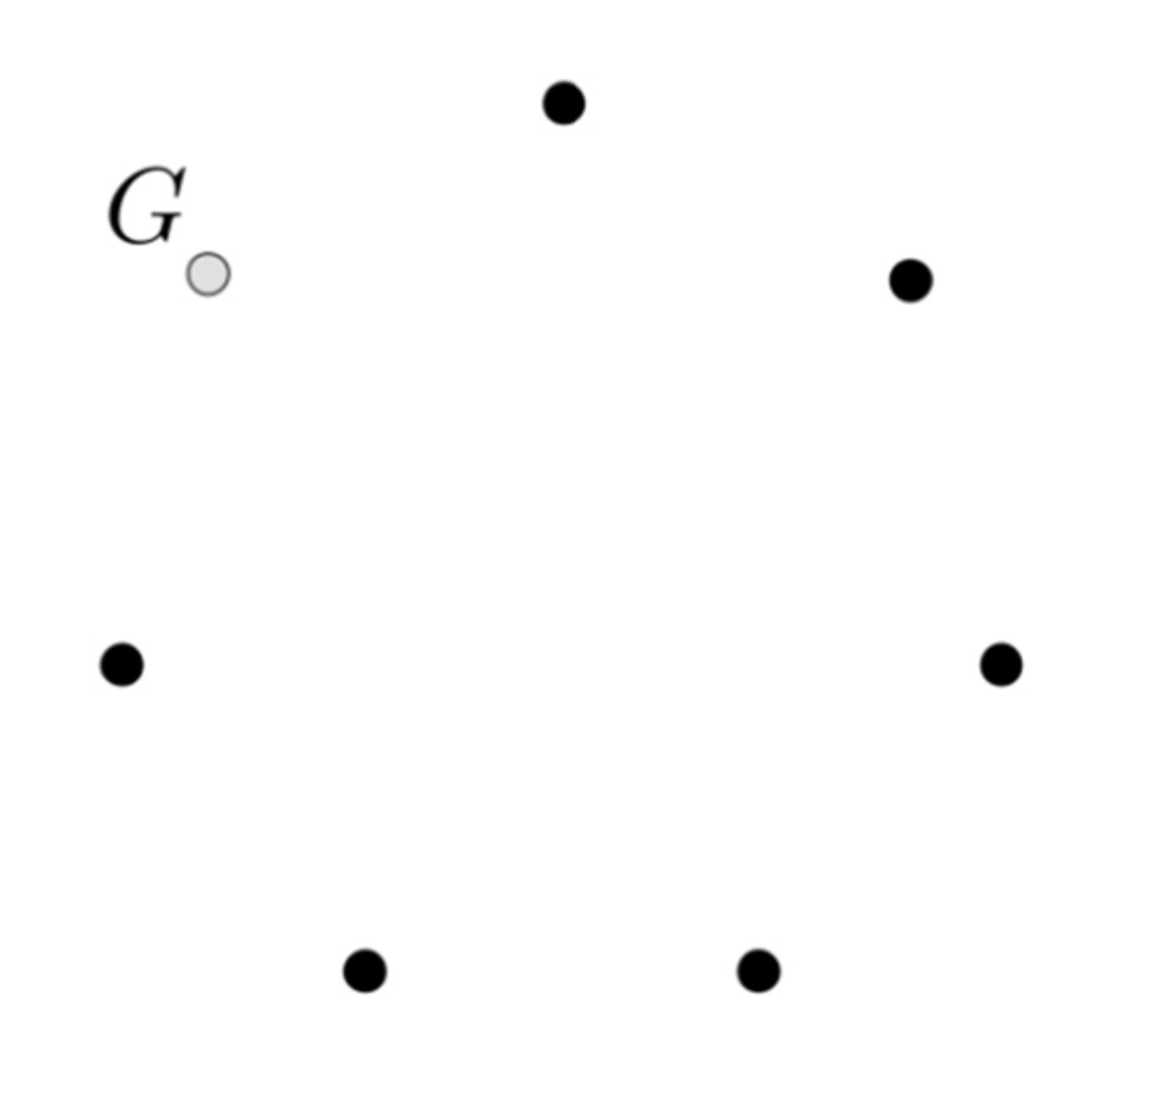
\includegraphics[width=0.4\linewidth]{kepek/Screenshot 2024-04-19 220001.png}
    \end{figure}

\vspace{\fill}

    \begin{flushright}
        \begin{tabular}{|>{\raggedright}M{6cm}|M{2cm}|M{2cm}|}
        \cline{2-3}
        \multicolumn{1}{c|} \
         & 
        \vspace{20pt}
         2 pont \cellcolor{black!20} & \cellcolor{black!20} \\[30pt]
        \hline
        \vspace{20pt}
        G ismerőseinek száma: 
        & 
        \vspace{20pt}
         1 pont \cellcolor{black!20} & \cellcolor{black!20} \\[30pt]
        \hline
        \end{tabular}
    \end{flushright}

\newpage

    \item
Oldja meg az alábbi egyenletet a valós számok halmazán!
Válaszát tizedes tört alakban adja meg! 

\[4^x=8\]


    \vspace{4cm}
    \begin{flushright}
        \begin{tabular}{|M{6cm}|M{2cm}|M{2cm}|N}
        \hline
         & 
        \vspace{20pt}
         2 pont \cellcolor{black!20} & \cellcolor{black!20} \\[30pt]
        \hline
        \end{tabular}
    \end{flushright}
    
    \item

Adja meg a [–3; 1] zárt intervallumon értelmezett \(x \mapsto |x|\) függvény értékkészletét!


    \vspace{\fill}
    \begin{flushright}
        \begin{tabular}{|M{6cm}|M{2cm}|M{2cm}|N}
        \hline
         & 
        \vspace{20pt}
         2 pont \cellcolor{black!20} & \cellcolor{black!20} \\[30pt]
        \hline
        \end{tabular}
    \end{flushright}

\newpage

\item
Máté ebben a tanévben hat dolgozatot írt matematikából. A dolgozataira kapott osztályzatok mindegyike egész szám (1, 2, 3, 4 vagy 5). A hat osztályzat között csak egy 3-as
van, az osztályzatok átlaga pedig 4,5.\\
Adja meg ezt a hat osztályzatot! 


    \vspace{4cm}
    \begin{flushright}
        \begin{tabular}{|M{6cm}|M{2cm}|M{2cm}|N}
        \hline
         & 
        \vspace{20pt}
         2 pont \cellcolor{black!20} & \cellcolor{black!20} \\[30pt]
        \hline
        \end{tabular}
    \end{flushright}

\item 
Az ábrán egy, a [0; 4] zárt intervallumon értelmezett függvény grafikonja látható.
Válassza ki a felsoroltak közül a függvény hozzárendelési szabályát! 


\[\text{A}:x\mapsto(x-2)^2+1\hspace{1cm}\text{B}:x\mapsto(x-2)^2-1\hspace{1cm}\text{C}:x\mapsto(x+2)^2+1\hspace{1cm}\text{D}:x\mapsto(x+2)^2-1\]

\vspace{\fill}
    \begin{flushright}
        \begin{tabular}{|M{6cm}|M{2cm}|M{2cm}|N}
        \hline
         & 
        \vspace{20pt}
         2 pont \cellcolor{black!20} & \cellcolor{black!20} \\[30pt]
        \hline
        \end{tabular}
    \end{flushright}



\end{enumerate}

\label{LastPage}~
\end{document}